\documentclass{standalone}

\usepackage{tikz}

\usetikzlibrary{fit, calc, shapes, matrix}

\begin{document}
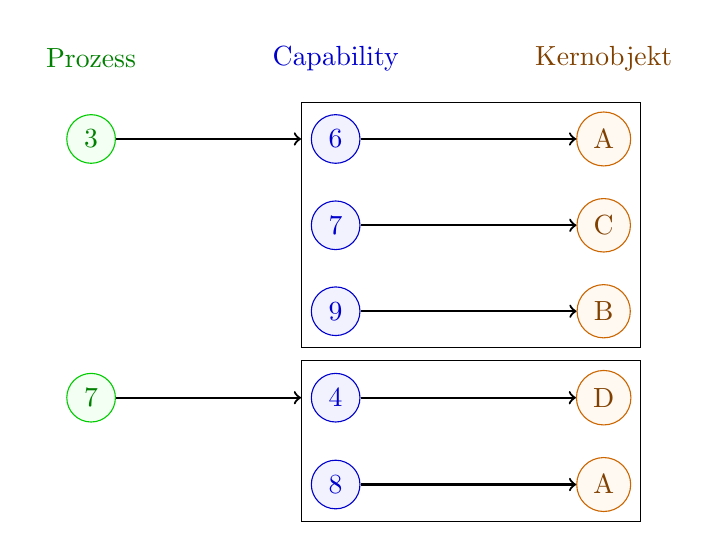
\begin{tikzpicture} [
  proc/.style={
    draw, circle, fill=green!5!white, text=green!50!black, draw=green!80!black
  },
  sel/.style={draw, circle, fill=blue!5!white, text=blue!80!black, draw=blue!80!black},
  ko/.style={
    draw, circle, fill=orange!5!white, text=orange!50!black, draw=orange!80!black},
  heading/.style={draw=none, fill=none, rectangle}
  ]
  \matrix[row sep=4mm, column sep=1.5cm] { 
    \node[proc, heading]{Prozess}; & \node[sel, heading]{Capability}; & \node[ko, heading]{Kernobjekt}; \\
    \node(p1)[proc]{3}; & \node(s11)[sel]{6}; & \node(k11)[ko]{A}; \\
                        & \node(s12)[sel]{7}; & \node(k12)[ko]{C}; \\
                        & \node(s13)[sel]{9}; & \node(k13)[ko]{B}; \\
    \node(p2)[proc]{7}; & \node(s21)[sel]{4}; & \node(k21)[ko]{D}; \\
                        & \node(s22)[sel]{8}; & \node(k22)[ko]{A}; \\
  };
  \node(s1)[fit=(s11) (s13) (k11) (k13), draw]{};
  \node(s2)[fit=(s21) (s22) (k21) (k22), draw]{};
  \begin{scope}[thick]
    \draw[->] (p1) -- (p1 -| s1.north west);
    \draw[->] (p2) -- (p2 -| s2.north west);
    \draw[->] (s11) -- (k11);
    \draw[->] (s12) -- (k12);
    \draw[->] (s13) -- (k13);
    \draw[->] (s21) -- (k21);
    \draw[->] (s22) -- (k22);
  \end{scope}
\end{tikzpicture}
\end{document}
